% Requires \usepackage{graphicx}. Figures are vector PDFs.
% Paths below assume this file's directory; add your project-relative prefix if needed.
\begin{figure*}[t]
  \centering
  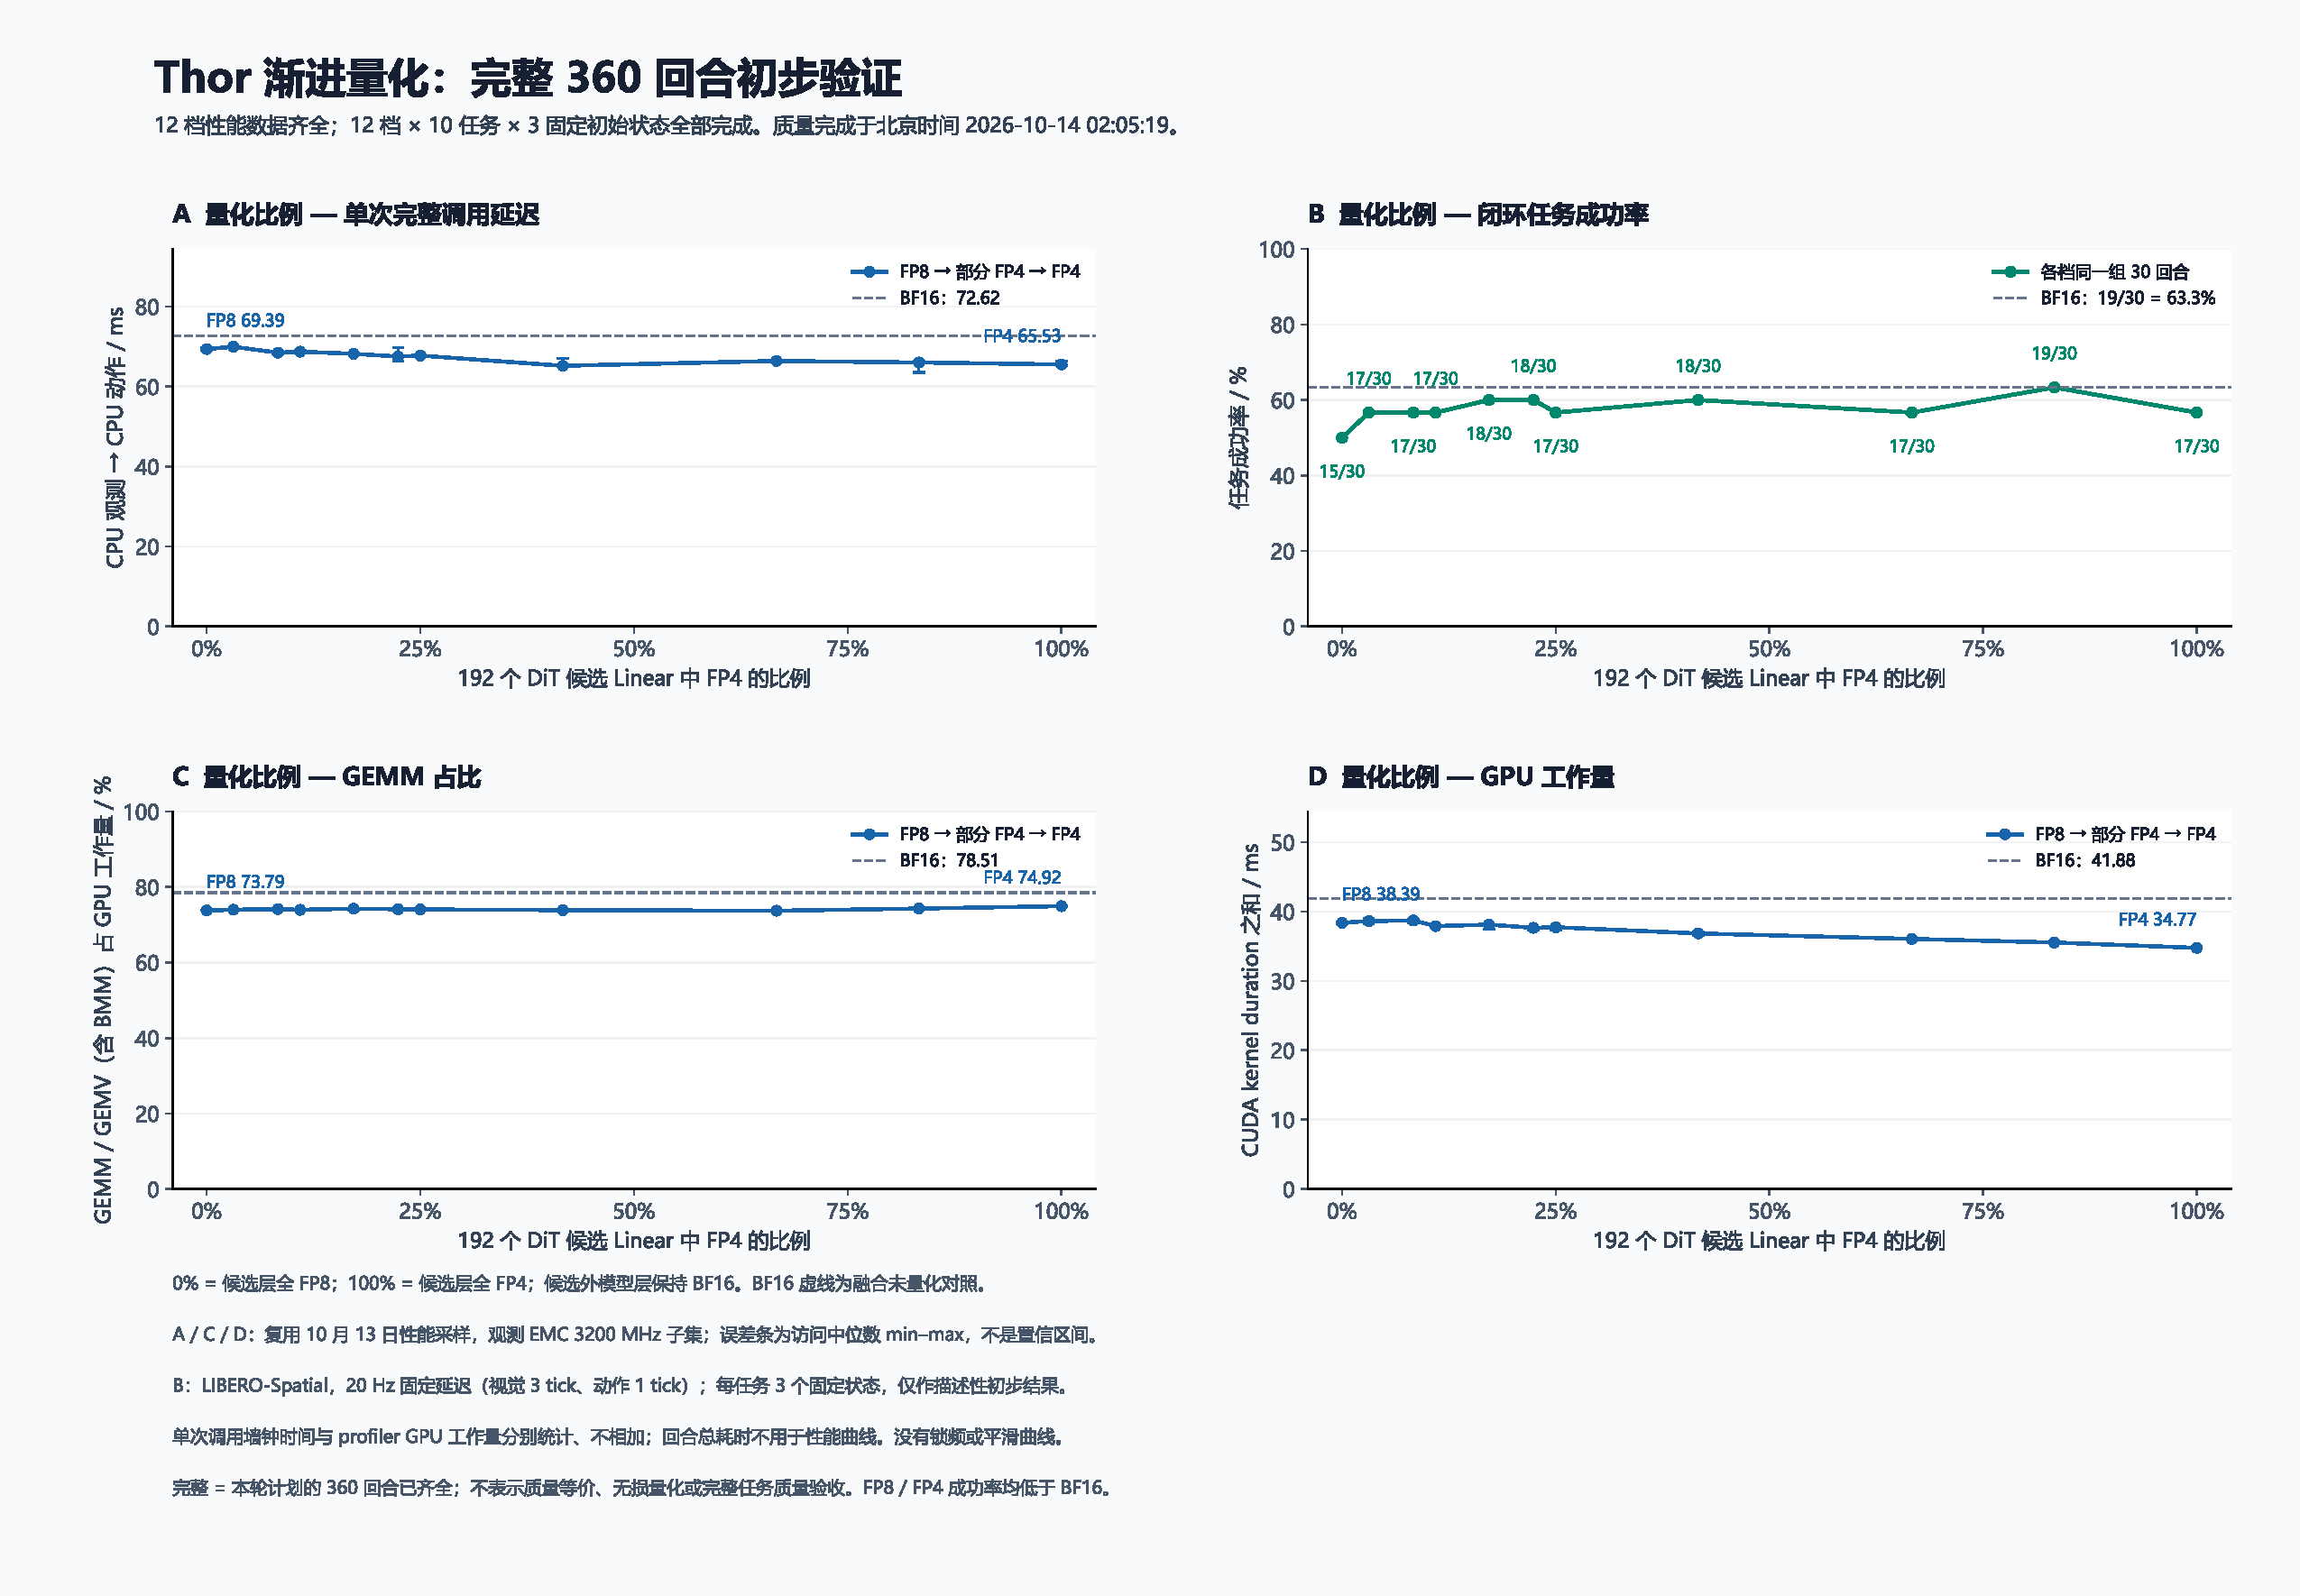
\includegraphics[width=\textwidth]{thor_progressive_complete.pdf}
  \caption{Thor progressive FP8-to-FP4 scan with the completed 360-episode pilot. The 11 tiers replace 0, 6, 16, 21, 33, 43, 48, 80, 128, 160, and 192 of 192 DiT candidate Linear layers with FP4; remaining candidates use FP8 and other model layers remain BF16. Dashed lines denote fused BF16. (A) Single complete-call wall latency. (B) Fixed-delay LIBERO-Spatial task success, 10 tasks times 3 fixed initial states per configuration. (C) GEMM-family share of profiled GPU duration, including BMM/GEMV. (D) Sum of GPU kernel durations. Performance uses the existing observed 3200 MHz EMC stratum: medians of visit medians, with min--max bars, not confidence intervals. Clocks were monitored without locking. Quality uses 20 Hz fixed delays of 3 visual and 1 action ticks and is separate from wall-clock deployment quality. Completing this small pilot does not establish quality equivalence or non-inferiority.}
  \label{fig:thor-progressive-complete}
\end{figure*}

\begin{figure*}[t]
  \centering
  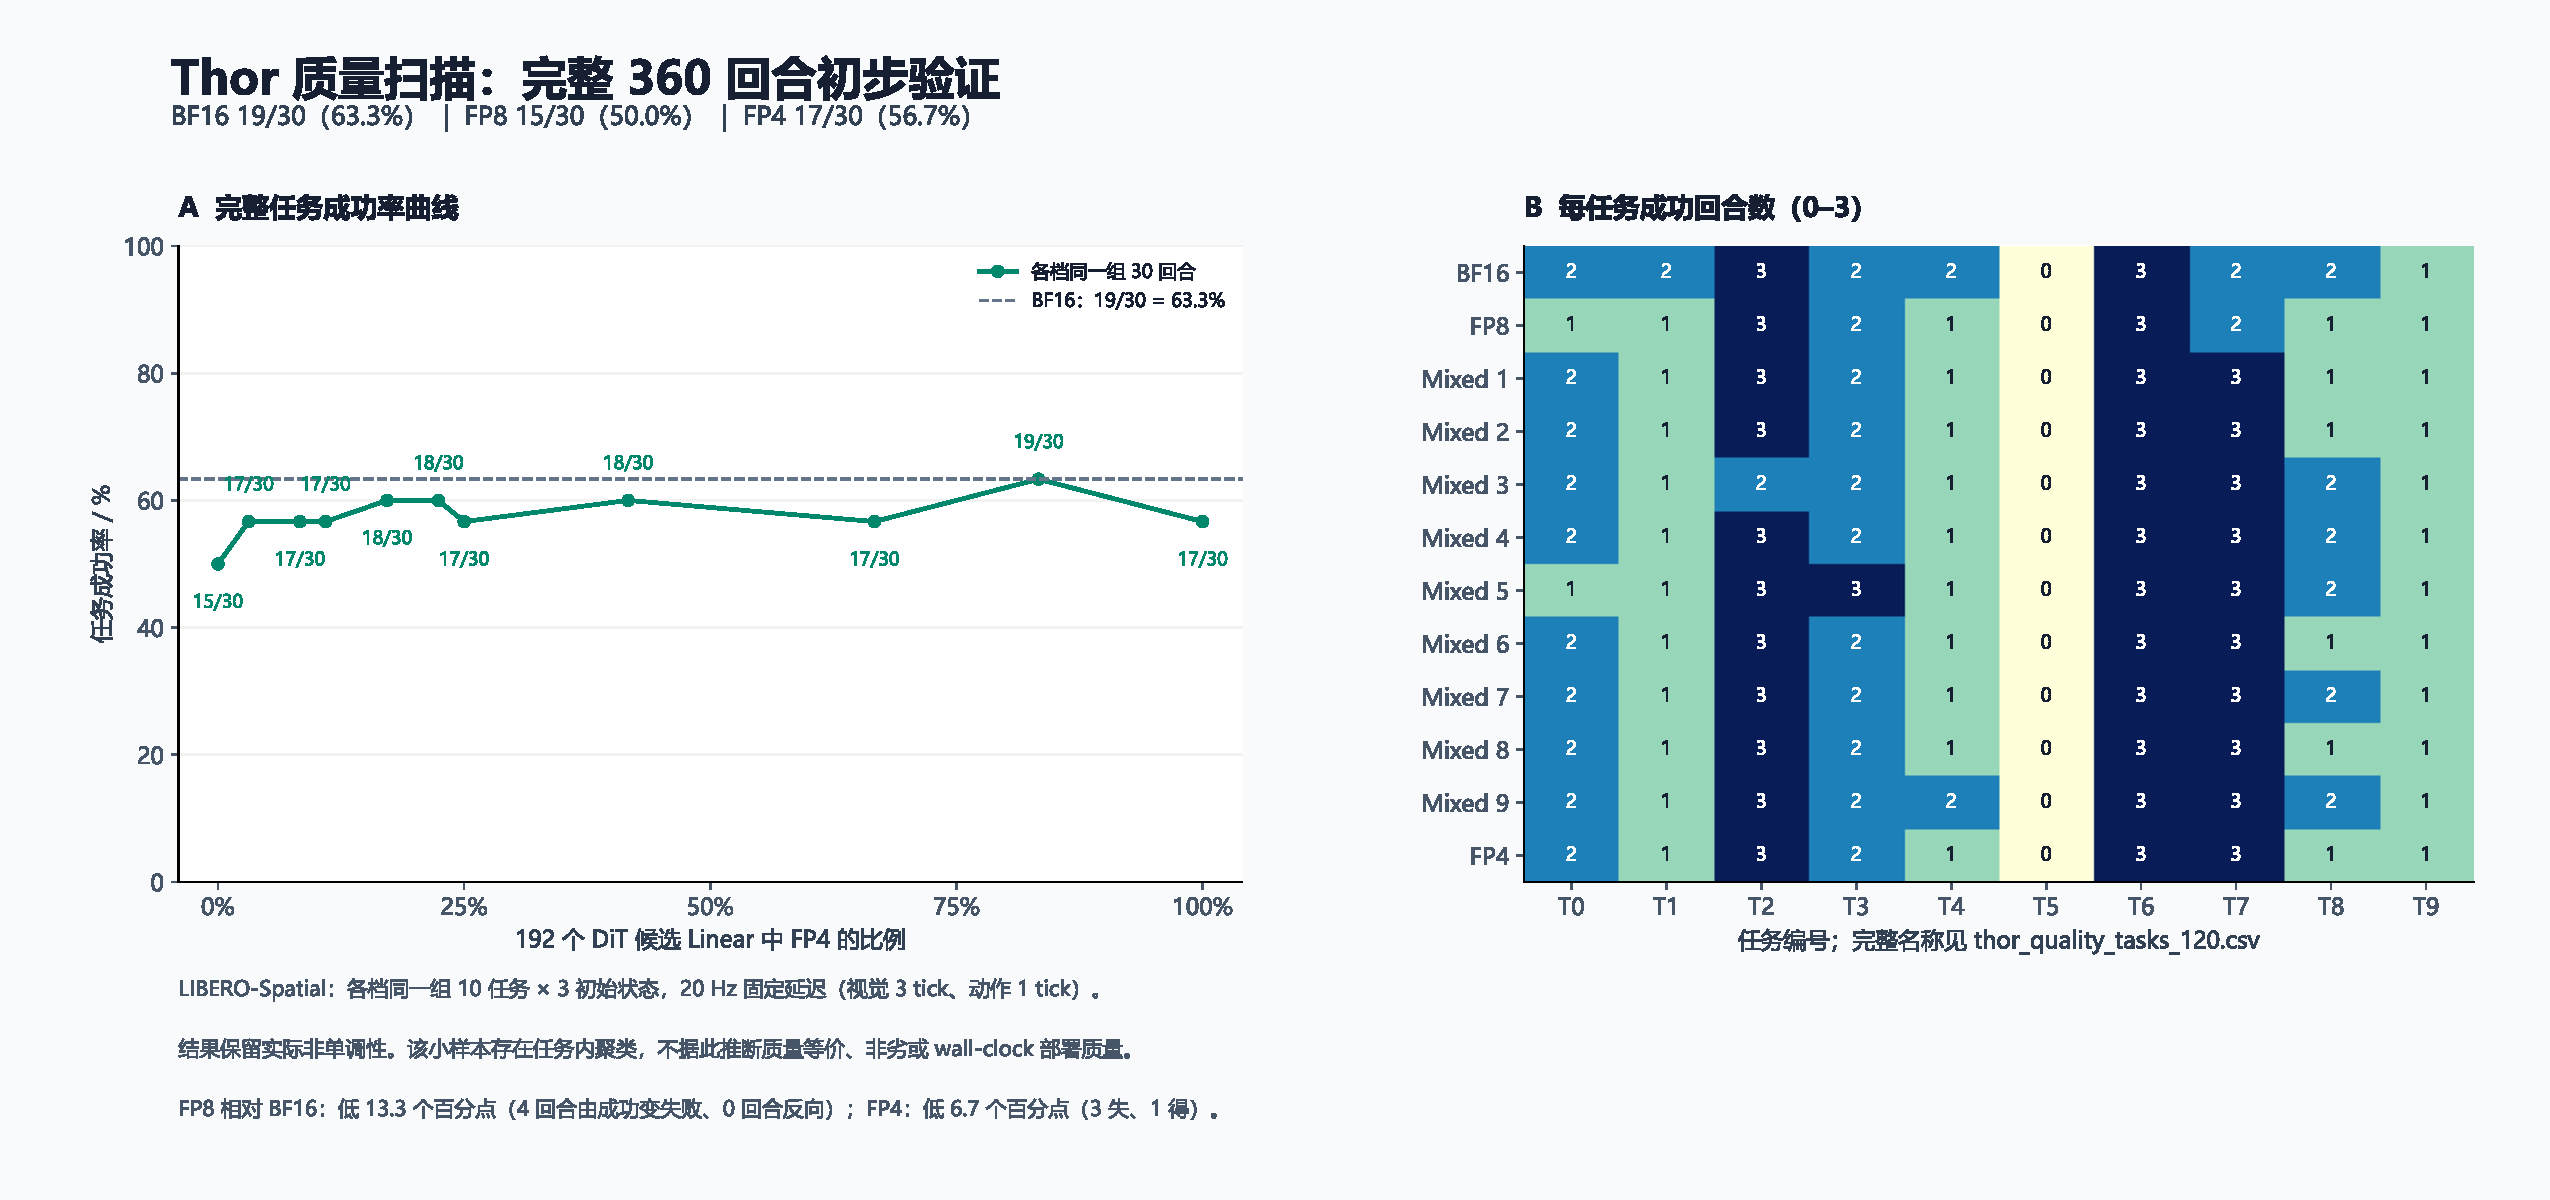
\includegraphics[width=\textwidth]{thor_quality_complete.pdf}
  \caption{Completed descriptive quality scan: 12 configurations with the same 30 task/initial-state pairs. Left: success rate versus FP4 candidate-layer fraction. Right: successes out of 3 for each task and configuration. BF16, FP8 and FP4 achieved 19/30, 15/30 and 17/30 successes, respectively. The three fixed states per task form a clustered pilot, not evidence of quality equivalence; no inferential intervals are shown.}
  \label{fig:thor-quality-complete}
\end{figure*}
